\documentclass[../main.tex]{subfiles}
\begin{document}
\subsection{Grandezze fisiche}
\begin{itemize}
    \item Grandezza fisica $\rightarrow \color{blue}m, \color{black}V, \color{Red}v, \color{black}l, p, \color{Red}a, \color{black}P, \color{blue}t, \color{black}R, A, f, E, \color{Red}F, \color{blue}T, s$
    \color{black}
    
    In \color{blue}blu \color{black}sono rappresentate le grandezze fondamentali mentre in \color{Red}rosso \color{black}le grandezze vettoriali, le grandezze non vettoriali sono chiamate scalari.
    \item Unità di misura $\rightarrow$ Ogni grandezza ha la sua unità di misura, il sistema internazionale (S.I.) stabilisce l'insieme di grandezze e unità di misura riconosciute a livello internazionale.
\end{itemize}
\begin{figure}[h]
    \centering
    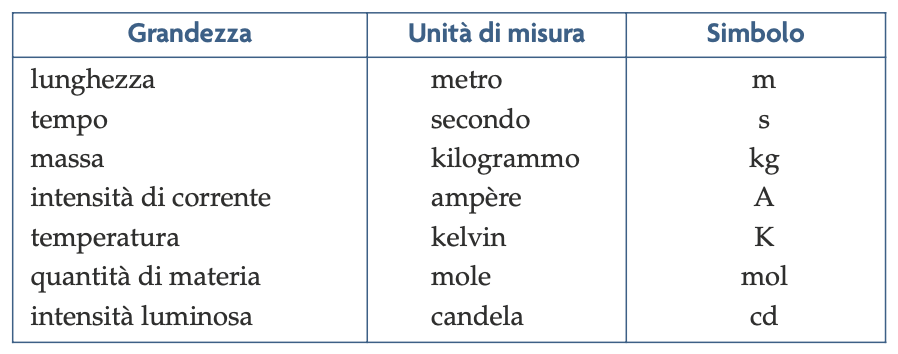
\includegraphics[width=0.8\textwidth]{images/unitaDiMisuraSI.png}
    \caption{Unità di misura fondamentali del SI}
\end{figure}

\subsection{Conversioni}
A prescindere dal sistema utilizzato, i multipli delle unità di base sono comuni. Per indicarli si usano prefissi standard che designano i multipli espressi tramite potenze di 10.
\begin{figure}[h]
    \centering
    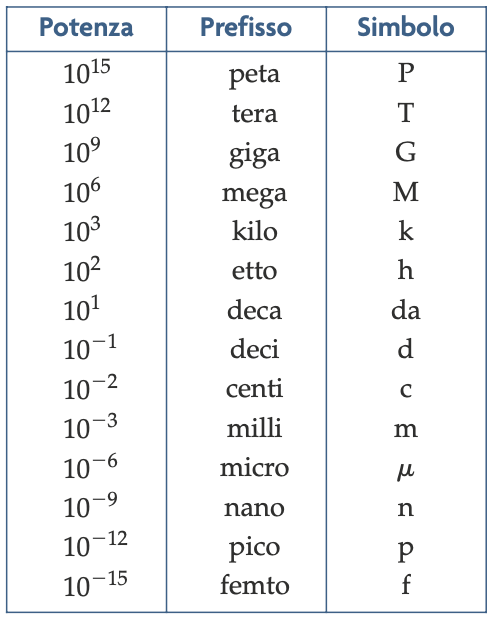
\includegraphics[width=0.4\textwidth]{images/prefissiStandard.png}
    \caption{Prefissi standard}
\end{figure}

Per noi è importante capire bene questa tabella per eseguire delle conversioni durante i problemi.

\textbf{Nota: }in casi in cui si abbiano unità di misura elevate a potenza bisogna moltiplicare per l'esponente lo spostamento, ad esempio:

\begin{center}
    $36dm^2 = \color{blue} 0.36\color{black}m^2$ e non $3.6m^2$   
\end{center}
oppure
\begin{center}
        $12.4\frac{kg}{dm^3}=12'400\frac{kg}{m^3}$ e non $124\frac{kg}{m^3}$
\end{center}

\subsection{Notazione scientifica}
La notazione scientifica consiste nel mantenere \textbf{solo le unità} di un numero e moltiplicarle per $10^n$, qualunque esso sia. Ecco alcuni esempi:
\begin{align*}
    65'000=6.5\cdot10^{\color{blue}4} \color{black} \\
    12'000'000=1.2\cdot10^{\color{blue}7} \color{black} \\
    0.00133=1.33\cdot10^{\color{blue}-3} \color{black} \\
    20=2\cdot10^{\color{blue}1} \color{black} \\
    10^6=1\cdot10^{\color{blue}6} \color{black}
\end{align*}
L'esponente \color{blue}n \color{black}rappresenta \textbf{l'ordine di grandezza} che, nota bene, non è $10^n$ ma soltanto $n$.
\vspace{1cm}
\subsection{Cifre significative}
Le cifre significative rappresentano le cifre conosciute con certezza in un numero, di seguito sono riportati alcuni valori con annesso il numero delle proprie cifre significative:
\begin{center}
    $37.5^\circ C \rightarrow$ 3 cifre significative
\end{center}
\begin{center}
    $37.55^\circ C \rightarrow$ 4 cifre significative
\end{center}
\begin{center}
    $53.01kg \rightarrow$ 4 cifre significative
\end{center}
\begin{center}
    $053.01kg \rightarrow$ 4 cifre significative, gli zeri a sinistra non contano
\end{center}
\begin{center}
    $53.0100kg \rightarrow$ 6 cifre significative, gli zeri a destra contano
\end{center}
\begin{center}
    $0.013k \rightarrow$ 2 cifre significative, potrei scriverlo come $1.3\cdot10^{-2}k$
\end{center}
\textbf{Nota: }il numero di cifre significative deve essere mantenuto anche quando si converte in notazione scientifica, in uno degli esempi appena fatti sarebbe quindi:
\begin{center}
    $53.0100kg=5.30100\cdot10^1kg$ (6 cifre significative)
\end{center}

\subsubsection{Operazioni aritmetiche}
Il numero di decimali di una grandezza ottenuta come somma o differenza di grandezze è uguale al minor numero di decimali presenti in ogni addendo.
$$
    12.47m+6.1m=18.57\approx18.6m
$$

Il numero di cifre significative di una grandezza ottenuta come risultato della moltiplicazione o divisione di grandezze è uguale al numero di cifre significative della grandezza conosciuta con minor precisione.
\begin{center}
    $6.79\cdot10=67.9\approx68$ Il numero più piccolo ha 2 cifre significative
\end{center}
oppure
$$
    \frac{3.11\cdot6.190}{2.111}=9.11932\approx9.12
$$
In caso ci fossero entrambi i tipi di operazioni quello che andremo a fare sarà svolgere ogni operazione singolarmente, approssimando alle dovute cifre significative, prima di continuare con la prossima operazione. Ecco un esempio:
$$
    \frac{12.75}{3.93}+6.2\approx3.24+6.2\approx9.4
$$

\pagebreak
\subsection{Analisi dimensionale}
In fisica, qualunque formula valida deve essere dimensionalmente consistente, i due termini dell'equazione della formula devono avere la stessa dimensione, di seguito è riportata una tabella con le dimensioni di alcune grandezze fisiche:
\begin{figure}[h]
    \centering
    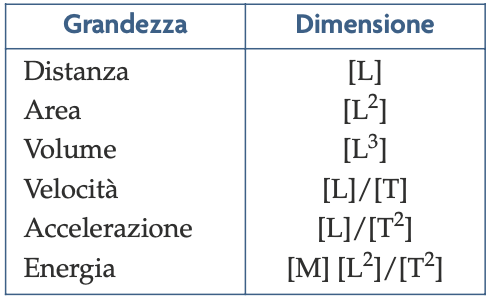
\includegraphics[width=0.5\textwidth]{images/dimensioni.png}
    \caption{Dimensione di alcune grandezze fisiche}
\end{figure}
Per verificare che una formula sia coerente dobbiamo quindi fare l'analisi dimensionale di essa, facciamo degli esempi per rendere meglio l'idea, di seguito viene eseguita l'analisi dimensionale di 3 formule (tutte corrette):

\begin{enumerate}[a)]
    \item \begin{align*}
        x&=v\cdot t \\
        \color{blue} m&\color{blue} \stackrel{?}{=} \frac{m}{s} \cdot s
    \end{align*}
    \item \begin{align*}
        x&=\frac{1}{2}\cdot at^2 \\
        \color{blue} m&\color{blue}\stackrel{?}{=} \frac{m}{s^2}
    \end{align*}
    \item \begin{align*}
        t&=(\frac{2x}{a})^{\frac{1}{2}} \\
        \color{blue} s&\color{blue}\stackrel{?}{=} (\frac{m}{m/s^2})^{\frac{1}{2}} \\
        \color{blue}s&\color{blue}\stackrel{?}{=}(s^2)^\frac{1}{2}
    \end{align*}
\end{enumerate}

\pagebreak
\subsection{Teoria degli errori}
Il valore di un errore in ambito ingegneristico è definito come \\$errore=valoreReale- valoreMisurato$. Gli errori possono essere sistematici oppure casuali. Per quanto riguarda gli errori sistematici, sono quegli errori che si ripetono con regolarità e che possiamo eliminare.

per determinare la precisione di uno strumento di misura e la percentuale di errori di esso ci sono diversi passaggi:
\begin{itemize}
    \item Media aritmetica \begin{align*}
        \overline{x}= x_m = \frac{x_1 + x_2 + \dots + x_n}{n} \\
        \text{oppure} \\
        \overline{x} = \frac{1}{n} \sum_{i=1}^{n} x_i
    \end{align*}
    \item Semidispersione \begin{align*}
        \Delta x = \frac{x_{max}-x_{min}}{2}
    \end{align*}
    \item Errore relativo \begin{align*}
        E_r = \frac{\Delta x}{\overline{x}}
    \end{align*}
    \item Errore percentuale \begin{align*}
        E_\%=E_r\cdot100
    \end{align*}
\end{itemize}

\subsubsection{Propagazione degli errori}
Le grandezze fisiche derivate non possono essere misurate direttamente, non possiamo misurare l'area di un tavolo in modo diretto, possiamo solo calcolarle misurando ad esempio base e altezza. Seguendo quanto vale per la teoria degli errori, è logico pensare che dovendo basarci su un set di più dati, quando si calcola una grandezza derivata gli errori si propagano su essa.

Per calcolare quindi il valore di errore di una grandezza derivata dobbiamo quindi affrontare il problema in modo diverso, ci sono due casi principali:
\begin{itemize}
    \item \textbf{Somma e differenza} \\
    Nel primo caso la grandezza indiretta $G$ è ottenuta come somma o differenza di due o più grandezze dirette $x$ e $y$ (ad esempio per il perimetro). 

    In questo caso $\Delta G = \Delta x + \Delta y$ e $E_r(G) = E_r(x)+E_r(y)$, poichè le grandezze si misurano con la stessa unità di misura è possibile sommare le semidisperioni.

    \item \textbf{Prodotto e rapporto} \\
    A differenza del caso precedente, non si possono sommare le semidispersioni in quanto aventi unità di misura diverse. Bisogna quindi affrontare il problema in un altro modo, sommando gli errori relativi che non hanno unità di misura. In questo caso valgono quindi le seguenti formule:
    \begin{align*}
        E_r(G) = E_r(x) + E_r(y) &= \frac{\Delta x}{x_m}+\frac{\Delta y}{y_m} \\
        E_r(G) &= \frac{\Delta G}{G_m} \\
        \Delta G = G_m \cdot E_r(G) &= G_m \cdot (\frac{\Delta x}{x_m}+\frac{\Delta y}{y_m})
    \end{align*}

    In questo caso calcoliamo quindi le singole semidispersioni e le singole medie, ricaviamo i singoli errori relativi e da essi calcoliamo il valore medio di $G$ e risaliamo a $\Delta G$.
\end{itemize}

\end{document}